% !TEX root = ../Hamiltonian_of_mean_force.tex
% Hero figure: 2x2 schematic
\begin{figure}[t]
\centering
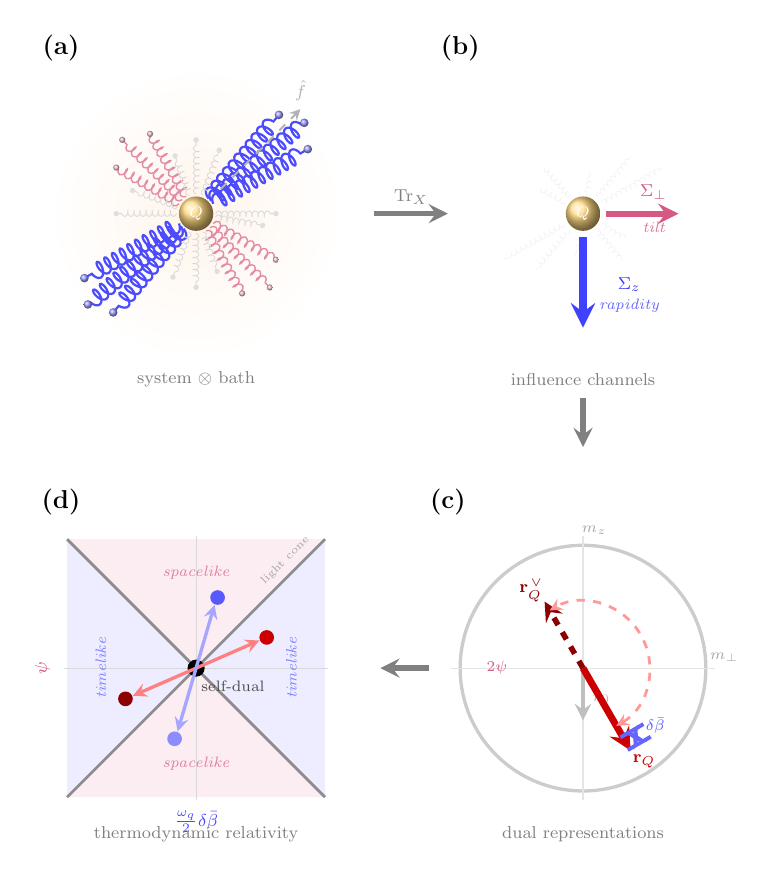
\begin{tikzpicture}[>=stealth, font=\small, scale=0.78, transform shape]

% ══════════════════════════════════════════════════════════════════════════════
% PANEL (a): System in anisotropic bath — top left
% ══════════════════════════════════════════════════════════════════════════════
\begin{scope}[shift={(0,4.7)}]
  \node[font=\bfseries\large] at (-2.2,2.7) {(a)};

  \shade[inner color=orange!8, outer color=white] (0,0) circle (2.4);

  \foreach \ang/\len in {30/2.1, 40/2.3, 50/2.1, 210/2.1, 220/2.3, 230/2.1} {
    \draw[blue!70, line width=0.8pt, decorate,
          decoration={coil, segment length=3.2pt, amplitude=2.8pt}]
      ({0.32*cos(\ang)},{0.32*sin(\ang)}) -- ({\len*cos(\ang)},{\len*sin(\ang)});
    \shade[ball color=blue!40] ({\len*cos(\ang)},{\len*sin(\ang)}) circle (0.07);
  }
  \foreach \ang/\len in {120/1.5, 135/1.7, 150/1.5, 300/1.5, 315/1.7, 330/1.5} {
    \draw[purple!45, line width=0.5pt, decorate,
          decoration={coil, segment length=2.8pt, amplitude=1.6pt}]
      ({0.32*cos(\ang)},{0.32*sin(\ang)}) -- ({\len*cos(\ang)},{\len*sin(\ang)});
    \shade[ball color=purple!25] ({\len*cos(\ang)},{\len*sin(\ang)}) circle (0.05);
  }
  \foreach \ang/\len in {0/1.3, 70/1.1, 90/1.2, 110/1.0,
                         160/1.1, 180/1.3, 250/1.1, 270/1.2, 290/1.0, 350/1.1} {
    \draw[gray!30, line width=0.3pt, decorate,
          decoration={coil, segment length=2.2pt, amplitude=1.0pt}]
      ({0.32*cos(\ang)},{0.32*sin(\ang)}) -- ({\len*cos(\ang)},{\len*sin(\ang)});
    \filldraw[gray!25] ({\len*cos(\ang)},{\len*sin(\ang)}) circle (0.035);
  }

  \shade[ball color=orange!60!yellow!50] (0,0) circle (0.28);
  \node[font=\scriptsize\bfseries, white] at (0,0) {$Q$};

  \draw[->, gray!60, dashed, line width=0.7pt] (0.4,0.4) -- (1.7,1.7);
  \node[gray!60, font=\footnotesize] at (1.7,2.0) {$\hat{f}$};

  \node[font=\footnotesize, text=black!50] at (0,-2.7) {system $\otimes$ bath};
\end{scope}

% ── Arrow (a)→(b) ──
\draw[->, line width=2pt, black!50] (2.9,4.7) --
  node[above, font=\footnotesize] {$\mathrm{Tr}_X$} (4.1,4.7);

% ══════════════════════════════════════════════════════════════════════════════
% PANEL (b): Two influence channels — top right
% ══════════════════════════════════════════════════════════════════════════════
\begin{scope}[shift={(6.3,4.7)}]
  \node[font=\bfseries\large] at (-2.0,2.7) {(b)};

  \foreach \ang/\len in {30/1.5, 50/1.2, 130/1.0, 150/0.8, 210/1.5, 230/1.2,
                         310/1.0, 330/0.8, 80/0.7, 260/0.7} {
    \draw[gray!12, line width=0.2pt, decorate,
          decoration={coil, segment length=2pt, amplitude=0.8pt}]
      ({0.35*cos(\ang)},{0.35*sin(\ang)}) -- ({\len*cos(\ang)},{\len*sin(\ang)});
  }

  \shade[ball color=orange!60!yellow!50] (0,0) circle (0.28);
  \node[font=\scriptsize\bfseries, white] at (0,0) {$Q$};

  \draw[->, blue!75, line width=2.8pt, shorten >=1pt] (0,-0.38) -- (0,-1.9);
  \node[blue!75, font=\footnotesize\bfseries] at (0.75,-1.15) {$\Sigma_z$};
  \node[blue!60, font=\scriptsize\itshape] at (0.75,-1.50) {rapidity};

  \draw[->, purple!65, line width=2.2pt, shorten >=1pt] (0.38,0) -- (1.6,0);
  \node[purple!65, font=\footnotesize\bfseries] at (1.15,0.35) {$\Sigma_\perp$};
  \node[purple!55, font=\scriptsize\itshape] at (1.15,-0.22) {tilt};

  \node[font=\footnotesize, text=black!50] at (0,-2.7) {influence channels};
\end{scope}

% ── Vertical arrow (b)→(c) ──
\draw[->, line width=2pt, black!50] (6.3,1.7) -- (6.3,0.9);

% PANEL (c): Dual Bloch vectors — bottom right
% r_Q in lower hemisphere, r_Q^vee flipped to upper hemisphere
% ══════════════════════════════════════════════════════════════════════════════
\begin{scope}[shift={(6.3,-2.7)}]
  \node[font=\bfseries\large] at (-2.2,2.7) {(c)};

  % Bloch circle
  \draw[black!20, line width=1.2pt] (0,0) circle (2.0);

  % Faint axes
  \draw[black!10] (-2.15,0) -- (2.15,0);
  \draw[black!10] (0,-2.15) -- (0,2.15);
  \node[font=\scriptsize, black!35] at (0.18,2.25) {$m_z$};
  \node[font=\scriptsize, black!35] at (2.30,0.18) {$m_\perp$};

  % ── Bare Gibbs vector (grey, along −z) ──
  \draw[->, gray!50, line width=1.6pt] (0,0) -- (0,-0.85);
  \node[gray!55, font=\footnotesize] at (0.30,-0.50) {$r_0$};

  % State coordinates
  \pgfmathsetmacro{\rQ}{1.55}
  \pgfmathsetmacro{\tiltDeg}{30}
  % r_Q: tilted into lower-right quadrant
  \pgfmathsetmacro{\mxQ}{\rQ*sin(\tiltDeg)}
  \pgfmathsetmacro{\mzQ}{-\rQ*cos(\tiltDeg)}
  % r_Q^vee: flipped through origin into upper-left (point reflection)
  \pgfmathsetmacro{\rQd}{1.25}
  \pgfmathsetmacro{\mxQd}{-\rQd*sin(\tiltDeg)}
  \pgfmathsetmacro{\mzQd}{\rQd*cos(\tiltDeg)}

  % ── Mean-force state r_Q (solid red, lower hemisphere) ──
  \draw[->, red!80!black, line width=2.5pt] (0,0) -- (\mxQ, \mzQ);
  \node[red!80!black, font=\footnotesize\bfseries] at ({\mxQ+0.22}, {\mzQ-0.18})
    {$\mathbf{r}_Q$};

  % ── Dual state r_Q^vee (dashed red, upper hemisphere) ──
  \draw[->, red!55!black, line width=2.0pt, dashed] (0,0) -- (\mxQd, \mzQd);
  \node[red!55!black, font=\footnotesize] at ({\mxQd-0.22}, {\mzQd+0.18})
    {$\mathbf{r}_Q^{\,\vee}$};

  % Blue bracket: radial difference δβ̄ (along the r_Q direction)
  \draw[blue!60, line width=1.4pt, |<->|]
    ({\rQd*sin(\tiltDeg)+0.18*cos(\tiltDeg)}, {-\rQd*cos(\tiltDeg)+0.18*sin(\tiltDeg)})
    -- ({\rQ*sin(\tiltDeg)+0.18*cos(\tiltDeg)}, {-\rQ*cos(\tiltDeg)+0.18*sin(\tiltDeg)});
  \node[blue!65, font=\scriptsize\bfseries] at
    ({0.5*(\rQ+\rQd)*sin(\tiltDeg)+0.55*cos(\tiltDeg)},
     {-0.5*(\rQ+\rQd)*cos(\tiltDeg)+0.55*sin(\tiltDeg)})
    {$\delta\bar\beta$};

  % Duality arc: sweeping from r_Q to r_Q^vee through the equator
  \draw[<->, red!40, line width=1.0pt, dashed]
    ({\rQ*0.7*sin(\tiltDeg)}, {\rQ*0.7*cos(\tiltDeg)*(-1)})
    arc ({-90+\tiltDeg}:{90+\tiltDeg}:{\rQ*0.7});
  \node[purple!65, font=\scriptsize\bfseries] at (-1.4, 0.0) {$2\psi$};

  \node[font=\footnotesize, text=black!50] at (0,-2.7) {dual representations};
\end{scope}


% ── Arrow (c)→(d) ──
\draw[->, line width=2pt, black!50] (3.8,-2.7) -- (3.0,-2.7);

% ══════════════════════════════════════════════════════════════════════════════
% PANEL (d): Minkowski diagram — bottom left
% ══════════════════════════════════════════════════════════════════════════════
\begin{scope}[shift={(0,-2.7)}]
  \node[font=\bfseries\large] at (-2.2,2.7) {(d)};

  \fill[purple!7] (-2.1,2.1) -- (0,0) -- (2.1,2.1) -- cycle;
  \fill[purple!7] (-2.1,-2.1) -- (0,0) -- (2.1,-2.1) -- cycle;
  \fill[blue!7] (-2.1,-2.1) -- (0,0) -- (-2.1,2.1) -- cycle;
  \fill[blue!7] (2.1,-2.1) -- (0,0) -- (2.1,2.1) -- cycle;

  \draw[black!45, line width=1.0pt] (-2.1,-2.1) -- (2.1,2.1);
  \draw[black!45, line width=1.0pt] (-2.1,2.1) -- (2.1,-2.1);

  \draw[black!15] (-2.15,0) -- (2.15,0);
  \draw[black!15] (0,-2.15) -- (0,2.15);

  \filldraw[black] (0,0) circle (0.13);
  \node[font=\scriptsize, black!70] at (0.6,-0.30) {self-dual};

  \node[blue!70, font=\footnotesize\bfseries] at (0,-2.5)
    {$\frac{\omega_q}{2}\delta\bar\beta$};
  \node[purple!70, font=\footnotesize\bfseries, rotate=90] at (-2.5,0) {$\psi$};

  \node[purple!50, font=\scriptsize\itshape] at (0,1.55) {spacelike};
  \node[purple!50, font=\scriptsize\itshape] at (0,-1.55) {spacelike};
  \node[blue!50, font=\scriptsize\itshape, rotate=90] at (1.55,0) {timelike};
  \node[blue!50, font=\scriptsize\itshape, rotate=90] at (-1.55,0) {timelike};

  \filldraw[red!80!black] (1.15,0.5) circle (0.11);
  \filldraw[red!55!black] (-1.15,-0.5) circle (0.11);
  \draw[<->, red!50, line width=1.2pt] (1.03,0.45) -- (-1.03,-0.45);

  \filldraw[blue!65] (0.35,1.15) circle (0.11);
  \filldraw[blue!45] (-0.35,-1.15) circle (0.11);
  \draw[<->, blue!35, line width=1.2pt] (0.3,1.03) -- (-0.3,-1.03);

  \node[black!35, font=\tiny, rotate=45] at (1.45,1.75) {light cone};

  \node[font=\footnotesize, text=black!50] at (0,-2.7)
    {thermodynamic relativity};
\end{scope}

\end{tikzpicture}
\caption{From anisotropic bath influence to thermodynamic relativity.
\textbf{(a)}~A qubit coupled to a harmonic bath; the coupling
$\hat{f}$ (dashed) makes the influence anisotropic.
\textbf{(b)}~After the partial trace, the environment collapses to two
channels: $\Sigma_z$ (blue, rapidity/temperature renormalisation) and
$\Sigma_\perp$ (purple, tilt).
\textbf{(c)}~The resulting mean-force state $\mathbf{r}_Q$ (solid) and its
dual $\mathbf{r}_Q^{\,\vee}$ (dashed), with the radial separation
$\delta\bar\beta$ (blue) and angular gap $2\psi$ (purple) shown explicitly.
\textbf{(d)}~These separations define the axes of a Minkowski metric in
thermal coordinates. Temperature renormalisation $\to$ timelike; tilt
$\to$ spacelike. The dual map is point reflection through the self-dual
origin ($\bullet$).}
\label{fig:minkowski_hero}
\end{figure}
